%%% ============================================================
%%% Exemplo de uso da classe LaTeX Ifes8 (modo revista) para
%%% a Revista Ifes Ciência, de acordo com as normas estabelecidas no
%%% documento "Normas para Apresentação de Trabalhos Acadêmicos e
%%% Científicos: Documento Impresso e/ou Digital", 9ª edição -- 2024.
%%%
%%% Autor da classe ifes8: Prof. Jefferson O. Andrade <jefferson.andrade@ifes.edu.br>
%%% Exemplo criado por Gustavo Cardoso Pimentel
%%% Data de criação: 2026-08-12 | Data de atualização: 2026-08-13
%%%
%%% ============================================================

\documentclass[revista,english]{ifes8}

% ---------------- Dados do artigo ----------------
\revistavolume{v.9n.1 2023}
\revistapaginas{XX-YY}
\revistadoi{YYYYYY}
\artigotitulo{PAPER TITLE}
\datasubmissao{XX/XX/XXXX}
\dataaceitacao{XX/XX/XXXX}
\datapublicacao{XX/XX/XXXX}

\begin{document}

%% ==================================================================
%% PÁGINA 1 -- Capa do artigo (faixa ISSN/DOI, banner, resumo
%% gráfico, título, autores, endereços e nota de submissão)
%% ==================================================================
\imprimircaparevista

\begin{graphicalabstract}
\textbf{<Insert here image of the Graphical Abstract}

\textbf{(texts within the images must be in English)>}

\vspace{8mm}

<Insert here the descriptive text of the Graphical Abstract (1 to 2 lines, in English)>

\vspace{4mm}

\textit{\textbf{Graphical Abstract: it is a figure that represents or illustrates a
synthesis of the entire work. It can be done in PowerPoint or any other program the
author desires.}}
\end{graphicalabstract}

\imprimirtituloartigo

\noindent Author 1 (insert only after
acceptance)\textsuperscript{1}\orcid*,
Author 2 (insert only after
acceptance),\textsuperscript{2}\orcid{} and
Author 3 (insert only after acceptance),\textsuperscript{1}

\noindent \textsuperscript{1}Address. Remember that the smallest unit used must be the
Department or Coordination (do not mention laboratory, group, postgraduate program
etc.), then the Institute (if any), then the University. Use always full text. Example:
Mechanical Engineering Coordination, Instituto Federal do Espírito Santo, Campus São
Mateus, 29032-540 São Mateus -- ES, Brazil.

\noindent \textsuperscript{2} In case of authors from another institute or another
campus of the institution, separate the authors by address.

\begin{flushright} * (insert the e-mail of the corresponding author) \end{flushright}

\imprimirdatasartigo

\vfill

\noindent\textbullet\quad Keep the ORCID logo (green dot) for authors who have ORCID.
Fill in as the example below: ORCID -- João D. de Almeida:
\url{https://orcid.org/0000-0012-3645-795X}

\newpage

%% ==================================================================
%% PÁGINA 2 -- Abstract e Keywords (coluna única)
%% ==================================================================
\noindent\textbf{Abstract:} The abstract structure consists of a single paragraph,
containing up to 250 words, Times New Roman font, size 11 - single spacing between
lines, justified. The abstract text must represent the content of the research, covering
the paper proposal, objectives, theoretical foundation/discussion, methodological
procedures and main results. It should not include bibliographic references. The verb
must be used in the active voice and in the third person singular (ABNT - NBR 6028).

\vspace{4mm}
\noindent\textbf{Keywords}: Word(s) that represent(s) the content of the document and
chosen from controlled vocabulary. Insert a maximum of five (5), written in lowercase
letters (except in case of first names or abbreviations), written in the language of the
text, separated by a semicolon and with a period after the last one.

\newpage

%% ==================================================================
%% CORPO DO ARTIGO -- INTRODUÇÃO até REFERÊNCIAS (2 colunas)
%% ==================================================================
\twocolumn
\noindent\textbf{1 INTRODUCTION (titles and subtitles are at the discretion of the
author(s) -- only when applicable)}

The introduction is a logical argumentative work that validates the need to carry out
the study. This is an initial part of the article in which the author(s), normally,
establish(es) a delimitation of the subject addressed, considering other research
already carried out, and presenting objectives, justification and other elements
necessary to situate the theme addressed in the proposal.

Research does not start from scratch, so it is important that the researcher does a
prior study of what has already been written about the subject he will address. Even if
it is an unprecedented field research, which evaluates a concrete, unknown situation in
a given location, someone or a group, somewhere, must have already carried out similar
research(es), or even complementary research(es) to certain aspects of the intended. The
search for such sources, whether documentary or bibliographic, becomes essential so that
there is no duplication of efforts.

In this space, you can present many topics.

\vspace{4mm}
\noindent\textbf{2 METHODOLOGICAL PROCESSES or MATERIALS AND METHODS (at the discretion
of the author)}

In this item, it is recommended to detail the procedures involved in developing the
paper, in order to ensure that readers are able to correctly interpret the results or
use the information to reproduce the study. Only the methodologies that will support the
results and conclusions are presented. In some cases, this section may be subdivided
into topics in order to facilitate reading and identification of specific methodological
aspects of the work in question.

\vspace{4mm}
\noindent\textbf{4 RESULTS AND DISCUSSION}

Item of fundamental importance in/for the paper, because it will guide the discussion,
and may even be one of the first parts to be read by the reader. Therefore, the
presentation should emphasize the most important aspects of the data collected,
corresponding to those that will be referenced and commented on in the discussion.
However, special attention should be paid to the rules for presenting tables and
illustrated illustrations (drawings, diagrams, flowcharts, photographs, graphs, maps,
organizational charts, plans, tables, portraits and others).

\vspace{4mm}
\noindent\textbf{5 CONCLUSION \& PERSPECTIVES}

Final part of the article, in which the conclusions corresponding to the objectives and
hypotheses are presented. Conclusions should be brief, synthetically recapitulating the
results of the research carried out. This is not always the final answer to a problem.
This way, it is possible to present new research proposals around the topic studied.

\vspace{4mm}
\noindent\textbf{ACKNOWLEDGMENT}

Acknowledgments and credits to financing institutions must appear at the end of the text
and before the References item.

\vspace{4mm}
\noindent\textbf{REFERENCES (Information on next page)}

\newpage
\noindent\textbf{THE FOLLOWING INFORMATION ARE GUIDELINES FOR FORMATTING THE FILE TO BE
SENT FOR SUBMISSION. PLEASE REMOVE BEFORE SENDING THE DOCUMENT.}

All paragraphs of the text must follow the following formatting standard: Times New
Roman 12 font, single spacing between lines, justified, with an indent of 1.25 cm on the
first line of each paragraph. There must be 6 pt spacing after each paragraph. The main
text (between the INTRODUCTION section and REFERENCES) must be arranged in 2 columns,
with a spacing between columns of 0.88 cm.

\vspace{2mm}
\noindent\textbf{1 SECTION TITLES MUST BE IN TIMES NEW ROMAN 12 FONT, UPPERCASE, BOLD,
JUSTIFIED. ALL TITLES MUST BE NUMBERED SEQUENTIALLY WITHOUT PUNCTUATION.}

\vspace{2mm}
\noindent 1.1 LEVEL 2 SUBTITLES MUST BE JUSTIFIED, IN TIMES NEW ROMAN FONT, SIZE 12,
UPPERCASE, WITHOUT BOLD.

\vspace{2mm}
\noindent\textbf{1.1.2 Level 3 subtitles must be justified, in Times New Roman font,
size 12, in bold and only the initial letter in capital letters or, in the case of
proper nouns, the first letters of each word in capital letters.}

\vspace{4mm}
\noindent\textbf{2 QUOTATIONS} (Standards according to NBR 10520:2023) - In quotations,
the names of the author's surname, the responsible institution or the title included in
the sentence must be in upper- and lower-case letters.

\vspace{2mm}
\noindent 2.1 DIRECT QUOTATION - Textual transcription of part of the consulted author's
work.

\vspace{2mm}
\noindent a. \textit{Quotations with up to three lines}: must be contained within double
quotation marks. Single quotation marks are used to indicate citation within the
citation. Examples:

Barbour (1971, p. 35) describes: ``O estudo da morfologia dos terrenos [...] ativos
[...].''

``Não se mova, faça de conta que está morta.'' (Clarac; Bonnin, 1985, p. 72).

According to Sá (1995, p. 27): ``[...] por meio da mesma `arte de conversação' que
abrange tão extensa e significativa parte da nossa existência cotidiana [...].''

\vspace{2mm}
\noindent b. \textit{Quotations longer than three lines}: must be highlighted with a 2
cm indentation from the left margin, with font smaller than the text used and without
quotation marks. Example:

\begin{list}{}{\leftmargin=2cm\rightmargin=0pt}
\item[]\sffamily\fontsize{10}{12}\selectfont
A teleconferência permite ao indivíduo participar de um encontro nacional ou regional
sem a necessidade de deixar seu local de origem. Tipos comuns de teleconferência incluem
o uso da televisão, telefone e computador. Através de audioconferência, utilizando a
companhia local de telefone, um sinal de áudio pode ser emitido em um salão de qualquer
dimensão (Nichols, 1993, p. 181).
\end{list}

\vspace{2mm}
\noindent 2.2 INDIRECT QUOTATION -- Text based on the work of the consulted author.
Example:

Diversos autores salientam a importância do ``acontecimento desencadeador'' no início de
um processo de aprendizagem (Cross, 1984; Knox, 1986; Mezirow, 1991).

\vspace{4mm}
\noindent\textbf{3 REFERENCES} (Standards according to NBR 6023:2018) - References must
be drawn up in single space, aligned to the left margin of the text and separated from
each other by a single-spaced blank line. When they appear in footnotes, they must be
aligned to the left margin of the text and, from the second line of the same reference,
below the first letter of the first word, so as to highlight the exponent and without
space between them.

\vspace{2mm}
\noindent 3.1 PRIVATE INDIVIDUAL - The author should be indicated by the last name, in
uppercase letters, followed by the first name and other last names, abbreviated or not,
as they appear in the document. In the case of multiple authors, the authors' names
should be separated by a semicolon, followed by a space.

\vspace{2mm}
\noindent 3.1.1 Regardless of the number of authors, all of them must be indicated.
Examples:

SOUZA, J. C.; PEREIRA, A. M. \textbf{Metodologia de trabalho.} 3. ed. São Paulo:
Estrela, 2011.

TAYLOR, Robert; LEVINE, Denis; MARCELLIN-LITTLE, Denis; MILLIS, Darryl.
\textbf{Reabilitação e fisioterapia na prática de pequenos animais.} São Paulo: Roca,
2008.

\vspace{2mm}
\noindent 3.1.3 Authors with Hispanic names, compound names, family relationships, and
surnames with prefixes should be indicated according to the following:

\vspace{2mm}
\noindent a) Hispanic surnames:

GARCÍA MÁRQUEZ, Gabriel. \textbf{O amor nos tempos do cólera.} 33. ed. Rio de Janeiro:
Record, 2008.

\vspace{2mm}
\noindent b) Degree of relationship:

ASSAF NETO, Alexandre. \textbf{Estrutura e análise de balanços:} um enfoque
econômico-financeiro. 8. ed. São Paulo: Atlas, 2007.

\vspace{2mm}
\noindent c) compound surnames:

SAINT-ARNAUD, Yves. \textbf{A pessoa humana:} introdução ao estudo da pessoa e das
relações interpessoais. São Paulo: Loyola, 1984. 154 p.

ESPÍRITO SANTO, Miguel Frederico de. \textbf{O Rio Grande de São Pedro entre a fé e a
razão:} introdução à história do Rio Grande do Sul. Porto Alegre: Martins Livreiro,
1999. 144 p.

\vspace{2mm}
\noindent d) surnames with prefixes:

O'CONNOR, Colin. \textbf{Roman bridges.} Cambridge: Cambridge University Press, 1998.
235 p.

LA TORRE, Massimo. \textbf{Two essays on liberalism and utopia.} Florence: European
University Institute, 1998. 45 p.

\vspace{4mm}
\noindent 3.2 LEGAL ENTITY - The works under the responsibility of a legal entity
(government agencies, companies, associations, amog others) are entered as known or as
highlighted in the document, either in full or in abbreviated form. Examples:

ASSOCIAÇÃO BRASILEIRA DE NORMAS TÉCNICAS. \textbf{ABNT NBR 14724:} Information and
documentation: Academic works: presentation. Rio de Janeiro: ABNT, 2011.

UNIVERSIDADE DE SÃO PAULO. \textbf{Catálogo de teses da Universidade de São Paulo,
1992.} São Paulo: USP, 1993. 467 p.

PETROBRAS. \textbf{Biocombustíveis:} 50 perguntas e respostas sobre este novo mercado.
Rio de Janeiro: PETROBRAS, 2007.

\vspace{4mm}
\noindent 3.3 MONOGRAPH ENTIRETY- Includes a book and/or booklet (manual, guide,
catalog, encyclopedia, dictionary, among others) and academic work (thesis,
dissertation, final project, among others).

\vspace{2mm}
\noindent 3.3.1 The essential elements for a book and/or booklet are: author, title,
subtitle (if any), edition (if any), place, publisher, and date of publication. When
necessary, supplementary elements are added to the reference to better identify the
document. Examples:

LUCK, Heloisa. \textbf{Liderança em gestão escolar.} 4. ed. Petrópolis: Vozes, 2010.

LUCK, Heloisa. \textbf{Liderança em gestão escolar.} 4. ed. Petrópolis: Vozes, 2010. 165
p., 18 cm. (Cadernos de gestão, v. 4). Bibliografia: p. 149-155. ISBN 978-85-3263-62-01.

\vspace{2mm}
\noindent 3.3.2 The essential elements for an academic work are: author, title, subtitle
(if any), year of deposition, type of work (thesis, dissertation, final project, and
others), degree (specialization, doctorate, among others), and course in parentheses,
academic affiliation, place, and date of presentation or defense. When necessary,
supplementary elements are added to the reference to better identify the document.
Examples:

AGUIAR, André Andrade de. \textbf{Avaliação da microbiota bucal em pacientes sob uso
crônico de penicilina e benzatina.} 2009. Tese (Doutorado em Cardiologia) -- Faculdade
de Medicina, Universidade de São Paulo, São Paulo, 2009.

ALVES, Daian Péricles. \textbf{Implementação de conceitos de manufatura colaborativa: um
projeto virtual.} 2008. Trabalho de Conclusão de Curso (Bacharelado em Engenharia
Industrial Mecânica) -- Universidade Tecnológica Federal do Paraná, Curitiba, 2008.

RODRIGUES, Ana Lúcia Aquilas. \textbf{Impacto de um programa de exercícios no local de
trabalho sobre o nível de atividade física e o estágio de prontidão para a mudança de
comportamento.} Orientador: Mario Ferreira Junior. 2009. 82 f. Dissertação (Mestrado em
Fisiopatologia Experimental) -- Faculdade de Medicina, Universidade de São Paulo, São
Paulo, 2009.

\vspace{4mm}
\noindent 3.3 ARTICLE, SECTION, AND/OR MATERIAL FROM A PERIODICAL PUBLICATION - Includes
parts of a periodical publication, article, communication, editorial, interview, review,
report, critique, and others.

\vspace{2mm}
\noindent The essential elements are: author, title of the article or material, subtitle
(if any), title of the periodical, subtitle (if any), place of publication, year and/or
volume number, issue number and/or edition, volume (if any), initial and final pages,
and date or period of publication. Whenever possible, add the
DOI as a supplementary element, and when necessary, other supplementary elements may be
added to the reference to better identify the document. Examples:

ROCKE, Hans; ROSS, Johanna C. Online catalogs for and by librarians. \textbf{Technical
Services Quarterly}, Greeley, v. 2, n. 3/4, p. 1-9, Spring/Summer 1985. DOI
10.1300/J124v02n03\_01.

DE LUCCA, Gabriella. Notas curtas. \textbf{Getulio}, São Paulo, ano 3, p. 9, jul./ago.
2009.

DOREA, R. D.; COSTA, J. N.; BATITA, J. M.; FERREIRA, M. M.; MENEZES, R. V.; SOUZA, T. S.
Reticuloperitonite traumática associada à esplenite e hepatite em bovino: relato de
caso. \textbf{Veterinária e Zootecnia}, São Paulo, v. 18, n. 4, p. 199-202, 2011. Supl.
3.

SEKEFF, Gisela. O emprego dos sonhos. \textbf{Domingo}, Rio de Janeiro, ano 26, n. 1344,
p. 30-36, 3 fev. 2002.

\vspace{4mm}
\noindent 3.4 ARTICLE, SECTION, AND/OR MATERIAL FROM AN ELECTRONIC PERIODICAL
PUBLICATION - References must adhere to the standards indicated for article and/or
materials from periodical publications, following section 3.3, with the addition
of the DOI (if available) and information related to the physical description of the
electronic medium (CD-ROM, online, and others). When dealing with online articles, in
addition to the essential and supplementary elements, you should record the electronic
address, preceded by the expression ``Available at: <(website description)>'' and the
access date, preceded by the expression ``Accessed on:'' (remembering that, except for
May, the other months should be abbreviated after the third letter. Examples: Dec.,
Feb.).

VIEIRA, Cássio Leite; LOPES, Marcelo. A queda do cometa. \textbf{Neo Interativa}, Rio de
Janeiro, n. 2, inverno 1994. 1 CD-ROM.

SILVA, M. M. L. Crimes da era digital. \textbf{Net}, Rio de Janeiro, nov. 1998. Seção
Ponto de Vista. Disponível em:
\url{http://www.brazilnet.com.br/contexts/brasilrevistas.htm}. Acesso em: 28 nov.
1998.

WINDOWS 98: o melhor caminho para atualização. \textbf{PC World}, São Paulo, n. 75, set.
1998. Disponível em: \url{http://www.idg.com.br/abre.htm}. Acesso em: 10 set. 1998.

DANTAS, José Alves et al. Regulação da auditoria em sistemas bancários: análise do
cenário internacional e fatores determinantes. \textbf{Revista Contabilidade \&
Finanças}, São Paulo, v. 25, n. 64, p. 7-18, jan./abr. 2014. DOI:
\url{http://dx.doi.org/10.1590/S1519-70772014000100002}. Disponível em:
\url{http://www.scielo.br/scielo.php?script=sci_arttext&pid=S1519-70772014000100002&lng=en&nrm=iso}.
Acesso em: 20 maio 2014.

\vspace{4mm}
\noindent 3.5 EVENTS - Works resulting from events (seminars, conferences, symposiums,
among others) are entered under the name of the event, in full and in uppercase letters,
followed by its occurrence number (if any), year, and location of the event, in the
language of the document. The occurrence number should be in Arabic numerals, followed
by a period.

CONGRESSO BRASILEIRO DE BIBLIOTECONOMIA E DOCUMENTAÇÃO, 10., 1979, Curitiba. Anais
[...]. Curitiba: Associação Bibliotecária do Paraná, 1979. 3 v.

SIMPÓSIO DE INSTRUMENTAÇÃO E IMAGENS MÉDICAS, 3., 2007, São Carlos. [Anais]. São Carlos,
SP: Escola de Engenharia de São Carlos-USP, 2007. 1 CD-ROM.

\vspace{4mm}
\noindent\textbf{4 HOW TO PRESENT:}

\vspace{2mm}
\noindent\textbf{Tables -} formed by vertical lines but with open ends, used to express
quantitative data. The title, in Times New Roman, size 12, should be inserted as close
as possible to the beginning of the table. Below the table, provide the source from
which the data was extracted, in font size 10, followed by a period. Tables can occupy 1
column if necessary.

\begin{center} Table 1: Costs and time spent on printing

\vspace{2mm}
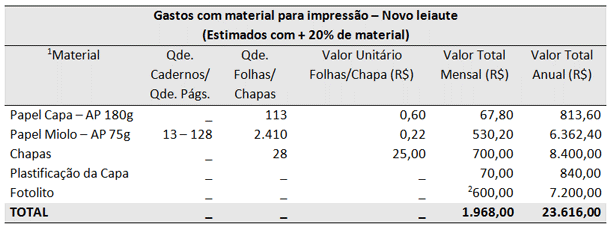
\includegraphics[width=\columnwidth]{pics/table_costs.png}

{\fontsize{10}{12}\selectfont Source: Nass (2003).} \end{center}

\vspace{2mm}
\noindent\textbf{Charts -} are generally formed by both vertical and horizontal lines
and should be closed at their ends. They are used to express qualitative data, unlike
tables. The title, in Times New Roman, size 12, should be inserted as close as possible
to the beginning of the chart. Below the chart, provide the source from which the data
was extracted, in font size 10, followed by a period. For the information within the
chart, use Times New Roman font, size 11. Charts can occupy 1 column if necessary.

\url{http://www.propesq.ufpe.br/anais/anais.htm}. Acesso em: 21 jan. 1997.

\begin{center} Table 1: Standards used in the preparation of a scientific article

\vspace{2mm}
\resizebox{\columnwidth}{!}{% \fontsize{11}{13}\selectfont
\begin{tabular}{|c|c|c|}
\hline
\textbf{Autor} & \textbf{Título} & \textbf{Data} \\
\hline
ABNT & NBR 6023: Elaboração de Referências & 2002 \\
\hline
ABNT & NBR 6028: Resumos & 2003 \\
\hline
ABNT & NBR: Citação em Documentos & 2002 \\
\hline
IBGE & Normas de Apresentação Tabular 3. ed & 1993 \\
\hline
\end{tabular}%
}

{\fontsize{10}{12}\selectfont Source: ABNT.NBR 6022 (2003, p. 1).} \end{center}

\vspace{2mm}
\noindent\textbf{Images -} a comprehensive category, including photographs,
illustrations, engravings, graphics, maps, flowcharts, etc. The title, in Times New
Roman, size 12, should be inserted as close as possible to the beginning of the image.
Below the image, provide the source from which the data was extracted, in font size 10,
followed by a period. Images can occupy 1 column if necessary.

\begin{center} Figure 1: Associação Brasileira de Normas Técnicas (ABNT)

\vspace{2mm}

\includegraphics[width=0.85\columnwidth]{pics/abnt_logo.png}

{\fontsize{10}{12}\selectfont Source: ABNT (2017).} \end{center}

\vspace{6mm} \begin{center}
\colorbox{red}{\textcolor{black}{\bfseries\fontsize{16}{18}\selectfont IMPORTANT}}
\end{center}

\vspace{4mm}
\noindent PLAGIARISM INFORMATION

The Ifes Ciência Journal conducts plagiarism and self-plagiarism checks on all
submissions. Therefore, any identification of plagiarism/self-plagiarism will result in
immediate rejection. Under no circumstances will the Ifes Ciência Journal accept
articles previously published on other platforms. If a work is found to be
plagiarized/self-plagiarized after its publication, it will be promptly removed from the
platform, and the author(s) will be notified and removed from the list of contributors
for the journal.

\end{document}